Το κεφάλαιο αυτό συνοψίζει όλη τη γνώση που δημιουργήθηκε από τη μελέτη των αλγορίθμων και την εξαγωγή αποτελεσμάτων. Παράλληλα, παρατηρώντας από ένα ευρύτερο πεδίο το θέμα δημιουργείται μια άλλη οπτική στην αντιμετώπιση του ζητήματος του εντοπισμού των μη τεχνικών απωλειών. Παρατηρούνται τα πλεονεκτήματα και τα μειονεκτήματα κάθε συστήματος, καθώς δίνεται βάση στο εύρος του πεδίου εφαρμογής του καθενός και στις δυνατότητές του. Τέλος διατυπώνονται κάποιες επισημάνσεις που έχουν ως κύριο μέλημα τη βελτιστοποίηση των συστημάτων.
\section{Σύγκριση αποτελεσμάτων}
Κάνοντας μια επισκόπηση στα αποτελέσματα, εύκολα παρατηρείται πως ο επιβλεπόμενος αλγόριθμος έχει την καλύτερη σχέση μεταξύ ποσοστού ευστοχίας στην εύρεση \en{DR} και ποσοστού λάθος προβλέψεων \en{FPR}. Αυτό ήταν αναμενόμενο από τα πρώτα στάδια της διπλωματικής, καθώς ο επιβλεπόμενος αλγόριθμος είναι ευρέως μελετημένος και είναι κοινά αποδεκτή η αποτελεσματικότητά του σε τέτοιου είδους δεδομένα. Παράλληλα, παρατηρείται πως ο αλγόριθμος μη επιβλεπόμενης μάθησης έχει υψηλότερο \en{DR} αλλά και υψηλότερο \en{FPR} στα όρια της κόκκινης γραμμής, που ορίστηκε στο 5\%. Με αυτό το σκεπτικό δημιουργήθηκε το ημι-επιβλεπόμενο σύστημα, ώστε να χαμηλώσει το \en{FPR} και να παραχθούν πιο σίγουρες προβλέψεις.\par
Τίθεται, λοιπόν, σαν άξονας αναφοράς ο επιβλεπόμενος αλγόριθμος που από τη μία έχει τα καλύτερα αποτελέσματα από τα άλλα συστήματα, αλλά από την άλλη είναι ο λιγότερο εφαρμόσιμος σε πραγματικά προβλήματα, λόγω της ανάγκης ύπαρξης δυαδικών χαρακτηριστικών. Συγκρίνοντας τα συστήματα με τον επιβλεπόμενο αλγόριθμο παρατηρούνται τα εξής:
\begin{itemize}
\item Το μη επιβλεπόμενο σύστημα κατέχει το σημαντικότερο πλεονέκτημα, που είναι η ευρεία και άμεση εφαρμογή του σε υπάρχοντα προβλήματα. Αυτό συμβαίνει, καθώς δεν απαιτεί κανενός είδους εκπαίδευση, αλλά μόνο εφαρμογή συμπαγών και αξιόπιστων κανόνων που να διαχωρίζουν τις δύο κλάσεις. Παράλληλα, λόγω της έλλειψης εκπαίδευσης, η δημιουργία του μοντέλου διαχωρισμού γίνεται ταχύτατα. Στα μειονεκτήματα του αλγορίθμου εντάσσεται η οριακή του γενική απόδοση. Το \en{FPR} είναι ακριβώς στα όρια ανοχής που ορίστηκαν (5\%), ενώ το \en{Accuracy} είναι λίγο χαμηλότερα από τα επιθυμητά επίπεδα (95\%).
\item Το ημι-επιβλεπόμενο σύστημα απαιτεί μόνο μικρό ποσοστό καταναλωτών για βελτιστοποίηση του ορίου επιλογής, γεγονός που το καθιστά πιο εύκολα εφαρμόσιμο από το επιβλεπόμενο σύστημα, αλλά λιγότερο εφαρμόσιμο από το μη επιβλεπόμενο σύστημα. Ουσιαστικά ο ημι-επιβλεπόμενος αλγόριθμος λειτουργεί σαν ενδιάμεση λύση σε όλα τα κριτήρια που έχουν τεθεί. Ειδικότερα, η απόδοσή του είναι βελτιωμένη με εξαιρετικά χαμηλό \en{FPR} και βελτιωμένο \en{Accuracy}. Παρόλο που το σύστημα φαίνεται να έχει σχετικά χαμηλό \en{DR}, αυτό εξισορροπείται από τη σιγουριά της πρόβλεψης που δίνεται από το \en{BDR}. Πιο συγκεκριμένα, όταν το σύστημα προβλέπει απάτη, είναι 80\% σίγουρο ότι πρόκειται για απάτη, ποσοστό που προσεγγίζει σε μεγάλο βαθμό το επιβλεπόμενο σύστημα.
\end{itemize}

\begin{center}
\begin{longtabu}  to 0.8\textwidth { | c || c | c | c | c | c |  }
 \hline
Σύστημα & \en{DR}  & \en{FPR} & \en{Accuracy} & \en{F1} &  \en{BDR} \\
 \hline
επιβλεπόμενο & 80.87 & 1.54 & 96.96 & 81.94 & 0.85 \\
μη-επιβλεπόμενο & 86.44	& 5.43 & 93.76 & 73.47 & 0.64\\
ημί-επιβλεπόμενο & 71.09 & 2.00 & 95.49 & 74.64 & 0.80\\
\hline
\caption{Σύγκριση συστημάτων}
\label{tab:comparesystems}
\end{longtabu}
\end{center}

Για την οπτικοποίηση αυτών των παρατηρήσεων δημιουργήθηκε ένα γράφημα δίνοντας βάση στο \en{Accuracy}, \en{F1 score} και \en{BDR}. Καθίσταται λοιπόν σαφές, πως η ημι-επιβλεπόμενη μάθηση βρίσκεται ακριβώς ανάμεσα στις επιδόσεις και στη χρηστικότητα του επιβλεπόμενου και μη επιβλεπόμενου συστήματος.

\begin{figure}[ht!]
\centering
 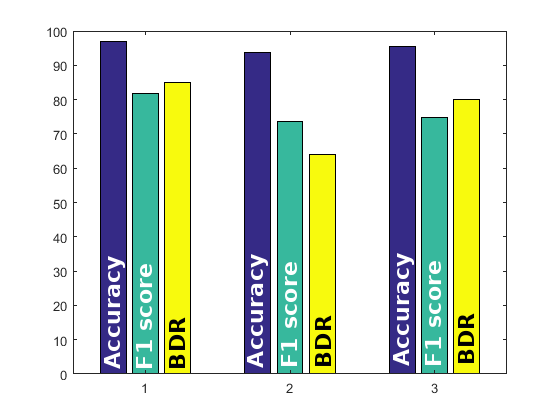
\includegraphics[width=90mm, height=60mm]{../../plots/comparison_systems.png}
 \caption{Σύγκριση συστημάτων}
\label{fig:comparisonsystem}
 \end{figure}
\section{Συμπερασματικές σημειώσεις}
Συνοψίζοντας χρήσιμες πληροφορίες που παρήχθησαν από αυτή τη μελέτη, γίνεται σαφές πως η ανίχνευση μη τεχνικών απωλειών με αλγορίθμους και συστήματα μηχανικής μάθησης είναι εφικτή και μάλιστα με υποσχόμενα αποτελέσματα. Οι γραμμικοί ταξινομητές μπορούν με μεγάλη επιτυχία να εντοπίσουν με ένα έτος εκπαίδευσης αν έχει εγκατασταθεί σύστημα αλλοίωσης των μετρήσεων. Η συσταδοποίηση των κανονικοποιημένων χρονοσειρών έχει επίσης πολύ καλά αποτελέσματα στον διαχωρισμό του κυρίως πληθυσμού από τον πληθυσμό καταναλωτών με ασυνήθιστες μετρήσεις. Το γεγονός αυτό είναι και ο λόγος που η συσταδοποίηση αποτέλεσε το βασικό συστατικό του μη επιβλεπόμενου και ημι-επιβλεπόμενου συστήματος. Χρησιμοποιήθηκαν δύο ειδών κανονικοποιήσεις, και διαπιστώθηκε πως η κανονικοποίηση σε εύρος [-1,1] ταιριάζει στις χρονοσειρές, ενώ σε εύρος [0,1] σε χαρακτηριστικά διαχωρισμού  με αραιούς πίνακες. Τέλος, καθίσταται σαφές πως η σύνδεση και αλληλεπίδραση διαφορετικών αλγορίθμων για τη δημιουργία μιας τελικής ταξινόμησης μπορεί να λειτουργήσει ικανοποιητικά, παρόλο που υπάρχουν περιθώρια δοκιμών και βελτιστοποιήσεων.
\section{Μελλοντική επέκταση}
Καταλήγοντας στην παρούσα διπλωματική αναλύθηκε ευρύ φάσμα αλγορίθμων μηχανικής μάθησης με επιτυχία, αλλά το ταξίδι για την βελτιστοποίηση συστημάτων μηχανικής μάθησης δεν έχει τέλος. Σε αυτό το σημείο αξίζει να αναφερθούν οι μελλοντικές επεκτάσεις της παρούσας έρευνας που πιστεύεται πως θα μπορούσαν να εξάγουν όμοια ή και καλύτερα αποτελέσματα στο πρόβλημα της ταξινόμησης. Πιο συγκεκριμένα, τα συστήματα που δημιουργήθηκαν θα μπορούσαν να συμπεριλάβουν τα εξής:
\begin{itemize}
\item \textit{Εφαρμογή ταξινόμησης σε περισσότερες από δύο κλάσεις}. Όλες οι ταξινομήσεις που δοκιμάστηκαν σε αυτή τη διπλωματική έγιναν σε δύο κλάσεις, την αρνητική και τη θετική. Παρ' όλα αυτά, τα αποτελέσματα έδειξαν ότι υπάρχουν καταναλωτές με ακανόνιστες χρονοσειρές που δεν έχουν ομοιότητες ούτε με τις πραγματικές χρονοσειρές (αρνητική κλάση), αλλά ούτε και με τις προσομοιωμένες απάτες (θετική κλάση). Για αυτό τον λόγο, θα είχε νόημα να δημιουργηθούν και άλλες κλάσεις που να ενδεικνύουν ιδιαίτερη καταναλωτική συμπεριφορά, αλλά όχι ρευματοκλοπή. Έτσι, θα ήταν εφικτή η περαιτέρω μείωση των εσφαλμένων προβλέψεων.
\item \textit{Εξερεύνηση τεχνικών ανίχνευσης ανωμαλιών}. Στην ανίχνευση ανωμαλιών στον ημι-επιβλεπόμενο αλγόριθμο χρησιμοποιήθηκε παραμετρική τεχνική Γκαουσιανού μοντέλου, καθώς είναι η συνηθέστερη τεχνική. Παρ' όλα αυτά, υπάρχουν ενδείξεις από τους γραμμικούς ταξινομητές πως οι παλινδρομήσεις των χρονοσειρών οδηγούν σε αξιόλογα αποτελέσματα. Θα είχε λοιπόν νόημα να δοκιμαστεί ανίχνευση ανωμαλιών βάσει του μοντέλου παλινδρόμησης. Παράλληλα, θα είχε ενδιαφέρον η προσέγγιση του αλγορίθμου από τη μη παραμετρική σκοπιά βάσει των ιστογραμμάτων και των συναρτήσεων πυρήνων, καθώς ήδη στην παρούσα διπλωματική υπάρχουν ενδείξεις με υποσχόμενα αποτελέσματα στο κεφάλαιο \ref{sec:histograms} και \ref{sec:RBFkernel} αντίστοιχα.
\item \textit{Ταξινόμηση βάσει πρόβλεψης μελλοντικής χρονοσειράς}. H ύπαρξη δεδομένων με μεγαλύτερο χρονικό ορίζοντα θα καθιστούσε δυνατή την καλύτερη κατανόηση των μεταβλητών που επηρεάζουν το επίπεδο της κατανάλωσης. Με αυτό τον τρόπο, θα μπορούσε κάθε καταναλωτής να αποκτά μια πρόβλεψη της κατανάλωσής του για το επόμενο έτος με μικρή απόκλιση από την πραγματική του κατανάλωση. Στην περίπτωση που η πρόβλεψη απέκλινε σημαντικά από την καταγραφείσα κατανάλωση, ο καταναλωτής θα θεωρούνταν ύποπτος. Η προσέγγιση αυτή θεωρείται υποσχόμενη, όπως έδειξε η στατιστική μελέτη που έγινε στο κεφάλαιο \ref{sec:statisticalexplore}.
\end{itemize} 